% questions.tex —— 1977 年·江苏南通卷 · 题目内容片段（无答案）
% 由 tools/generate_projects.py 依来源总账自 1977/1977_数学真题_江苏南通_试题.md 生成，勿手改（改源 MD 后重跑）


\gkpart{江苏省南通地区（试点）}

\begin{gktip}
\textbf{来源说明}：本题面依据固定源 PDF《1977 江苏南通》第 1—6 页逐题转录。源卷标题为「江苏省南通地区（试点）」，副题注明「共十题，每题 10 分」。固定源是题面与解答连续排印的书籍扫描（书籍页码 118—122），本文件只转录题面，解答经对照复算后写入答案要点与解析正文。原卷无文理分科说明，无附加题、参考题。题 1、题 2 的两个小问原卷以「1.」「2.」编号，本库按小问格式统一转写为（1）（2）。
\end{gktip}

\par\medskip

\begin{question}
\gkti{1}\textbf{（10 分）} 回答下列问题：

（1） 当 $a$ 为何值时，$2a>a$；当 $a$ 为何值时，$2a=a$；当 $a$ 为何值时 $2a<a$。

（2） 当 $x$ 为何值时，$|x|=x$。

\end{question}
\begin{question}
\gkti{2}\textbf{（10 分）} 写出下列函数的自变量 $x$ 的取值范围（在实数范围内）；

（1） $y=\dfrac{1}{2-x}$

（2） $y=\sqrt{2x-1}$

\end{question}
\begin{question}
\gkti{3}\textbf{（10 分）} 计算

\nopagebreak[4]
\[
\left(\frac{2}{3}\right)^{2}+(-5.8)^{0}-\left(\frac{8}{27}\right)^{-\frac{2}{3}}+\left(\frac{1}{2}\right)^{-2}.
\]

\end{question}
\begin{question}
\gkti{4}\textbf{（10 分）} $k$ 为何值时，方程 $x^{2}-2kx+4=0$ 有两个相等的实数根？并求出这方程的根。

\end{question}
\begin{question}
\gkti{5}\textbf{（10 分）} 已知 $\sin\alpha=\dfrac{3}{5}$（$90^\circ<\alpha<180^\circ$），求 $\cos\alpha$，$\operatorname{tg}\alpha$，$\operatorname{ctg}\alpha$。

\end{question}
\begin{question}
\gkti{6}\textbf{（10 分）} 试写出抛物线 $y=1+4x-2x^{2}$ 的顶点坐标，对称轴方程和函数 $y$ 的极值。

\end{question}
\begin{question}
\gkti{7}\textbf{（10 分）} 解方程

\nopagebreak[4]
\[
\frac{\lg 2x}{\lg (x-4)}=2.
\]

\end{question}
\begin{question}
\gkti{8}\textbf{（10 分）} 求 $200$ 以内的能被 $6$ 整除的所有自然数的和。

\Needspace{0.4\textheight}
\end{question}
\begin{question}
\gkti{9}\textbf{（10 分）} 已知正四棱锥底面边长为 $12\,\mathrm{cm}$，高为 $2\sqrt{7}\ \mathrm{cm}$，求它的侧棱。

\begin{gktip}
原源 PDF 第 5 页附有正四棱锥及其高、底面对角线的示意图；LaTeX 版按源图重绘。
\end{gktip}
\nopagebreak[4]
\begin{center}% 1977 年江苏南通卷第九题：正四棱锥 P-ABCD（P 顶点、O 底面中心），
% 高 PO 与底面对角线 AC 为虚线（按源卷第 5 页布局）
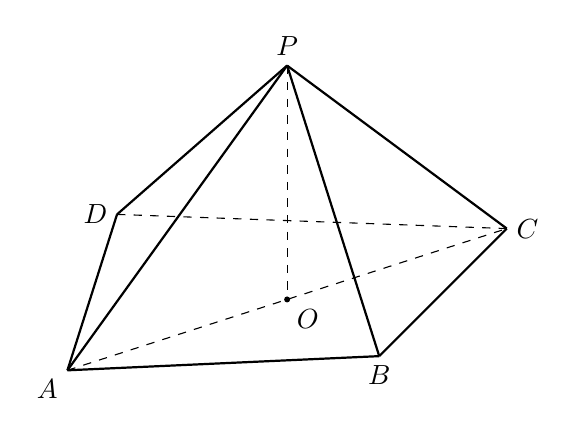
\begin{tikzpicture}[scale=0.9]
  \coordinate (A) at (0,0);
  \coordinate (B) at (4.4,0.2);
  \coordinate (C) at (6.2,2.0);
  \coordinate (D) at (0.7,2.2);
  \coordinate (P) at (3.1,4.3);
  \coordinate (O) at (3.1,1.0);
  \draw[thick] (P)--(A);
  \draw[thick] (P)--(B);
  \draw[thick] (P)--(C);
  \draw[thick] (P)--(D);
  \draw[thick] (A)--(B);
  \draw[thick] (B)--(C);
  \draw[thick] (D)--(A);
  \draw[dashed] (D)--(C);
  \draw[dashed] (A)--(C);
  \draw[dashed] (P)--(O);
  \fill (O) circle (1.2pt) node[below right] {$O$};
  \node[above] at (P) {$P$};
  \node[below left] at (A) {$A$};
  \node[below] at (B) {$B$};
  \node[right] at (C) {$C$};
  \node[left] at (D) {$D$};
\end{tikzpicture}
\end{center}
\nopagebreak[4]
\Needspace{0.4\textheight}
\end{question}
\begin{question}
\gkti{10}\textbf{（10 分）} 两根钢绳悬吊货物时，两条钢绳与铅垂线的夹角分别为 $\alpha$ 和 $\beta$，货物的重量为 $P$，试用表达式分别写出钢绳所承受的拉力 $F_1$ 和 $F_2$

\begin{gktip}
原源 PDF 第 5 页附有两条钢绳拉力与重力的受力示意图（图上编有 1、2、3、4 号角）；LaTeX 版按源图重绘。
\end{gktip}
\nopagebreak[4]
\begin{center}% 1977 年江苏南通卷第十题：两根钢绳悬吊货物的受力示意（按源卷第 5 页布局）：
% 结点处 F1（左上）、F2（右上）两条拉力与竖直向下重力 P，上方虚线把 F1、F2
% 作用线延长到竖直线交成力三角形，1、2 号角在结点处，3 号角在顶点处，4 号角在 F1 箭头端处
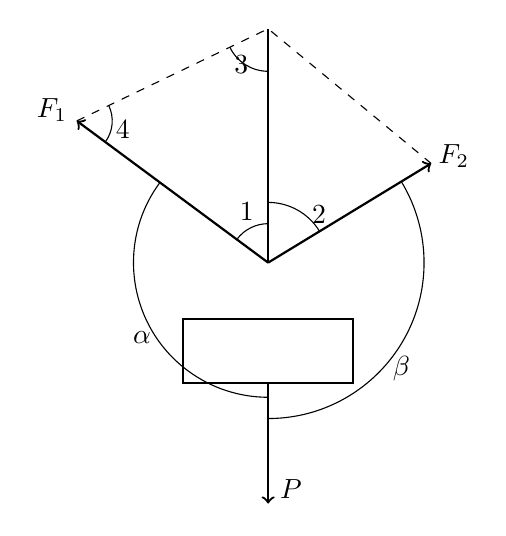
\begin{tikzpicture}[scale=0.9]
  \coordinate (K) at (0,0);
  \coordinate (T) at (0,3.3);
  \coordinate (L) at (-2.7,2.0);
  \coordinate (R) at (2.3,1.4);
  \draw[thick,->] (0,0)--(L);
  \node at (-3.05,2.15) {$F_1$};
  \draw[thick,->] (0,0)--(R);
  \node at (2.62,1.5) {$F_2$};
  \draw[thick] (0,0)--(T);
  \draw[dashed] (L)--(T);
  \draw[dashed] (R)--(T);
  \draw[thick] (-1.2,-0.8) rectangle (1.2,-1.7);
  \draw[thick,->] (0,-1.7)--(0,-3.4);
  \node at (0.32,-3.2) {$P$};
  \draw (90:0.55) arc[start angle=90, end angle=143.5, radius=0.55];
  \node at (-0.3,0.72) {$1$};
  \draw (90:0.85) arc[start angle=90, end angle=31.3, radius=0.85];
  \node at (0.72,0.68) {$2$};
  \begin{scope}[shift={(0,3.3)}]
    \draw (205.7:0.6) arc[start angle=205.7, end angle=270, radius=0.6];
  \end{scope}
  \node at (-0.38,2.8) {$3$};
  \begin{scope}[shift={(-2.7,2.0)}]
    \draw (25.7:0.5) arc[start angle=25.7, end angle=-36.5, radius=0.5];
  \end{scope}
  \node at (-2.05,1.88) {$4$};
  \draw (143.5:1.9) arc[start angle=143.5, end angle=270, radius=1.9];
  \node at (-1.78,-1.05) {$\alpha$};
  \draw (270:2.2) arc[start angle=270, end angle=391.3, radius=2.2];
  \node at (1.88,-1.5) {$\beta$};
\end{tikzpicture}
\end{center}
\nopagebreak[4]

\end{question}